% Fig. — Workup overview. Full width; shared workflow type scale.
\documentclass[tikz,border=1.5pt]{standalone}
\usepackage[T1]{fontenc}
\usepackage{lmodern}
\usepackage{helvet}
\renewcommand{\familydefault}{\sfdefault}
\usepackage{tikz}
\usetikzlibrary{arrows.meta,calc}

\definecolor{ojblue}{HTML}{0072B2}
\definecolor{ojbluedark}{HTML}{005080}
\definecolor{ojbluetint}{HTML}{EBF4FA}
\definecolor{cardbg}{HTML}{FFFFFF}
\definecolor{ink}{HTML}{0F172A}

\newcommand{\wffont}{\sffamily\fontsize{7.75}{9.0}\selectfont}
\newcommand{\wfleg}{\sffamily\fontsize{7.25}{8.25}\selectfont\bfseries}

\begin{document}
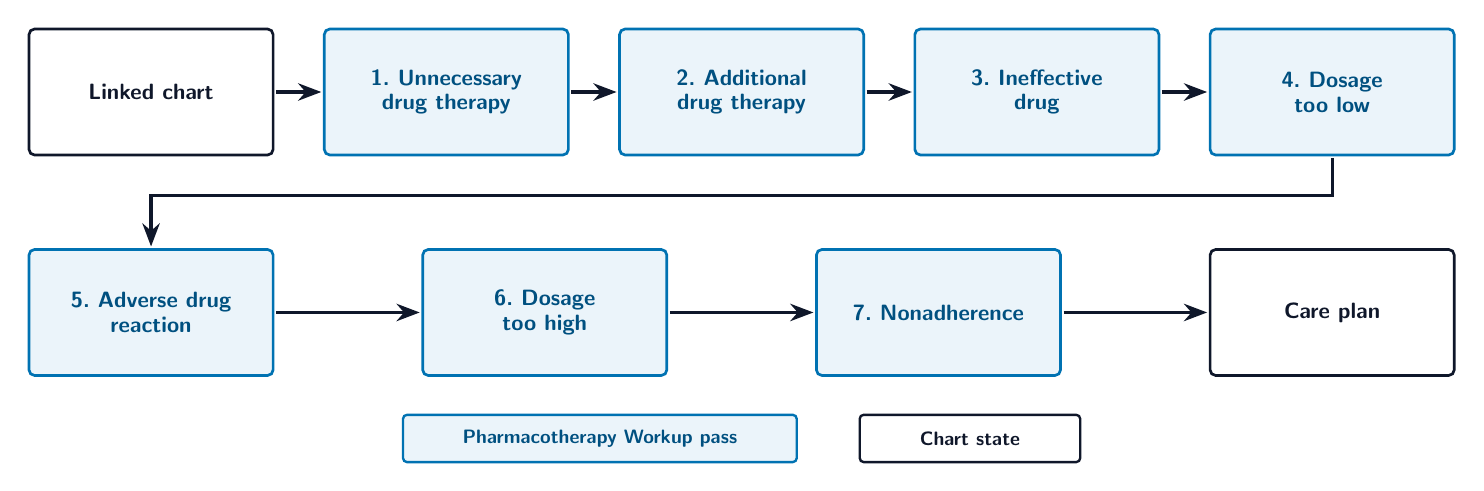
\begin{tikzpicture}[x=1mm,y=1mm,>=Stealth,font=\wffont,text=ink,
  every node/.style={align=center}]
  \tikzset{
    box/.style={
      draw, line width=0.34mm, rounded corners=0.7mm, align=center,
      minimum height=16mm, inner sep=0.55mm,
      font=\wffont\bfseries
    },
    pass/.style={box, draw=ojblue, fill=ojbluetint, text=ojbluedark,
                 text width=29mm, minimum width=31mm},
    state/.style={box, draw=ink, fill=cardbg, text=ink,
                  text width=29mm, minimum width=31mm},
    arr/.style={->, line width=0.42mm, draw=ink, shorten >=0.6pt, shorten <=0.6pt},
    leg/.style={
      draw, line width=0.30mm, rounded corners=0.5mm, align=center,
      minimum height=6mm, inner sep=0.4mm,
      font=\wfleg
    }
  }

  % Top row: centers 15.5 .. 165.5 (pitch 37.5), content center 90.5
  \node[state] (linked) at (15.5,28) {Linked chart};
  \node[pass] (p1) at (53.0,28) {1.~Unnecessary\\drug therapy};
  \node[pass] (p2) at (90.5,28) {2.~Additional\\drug therapy};
  \node[pass] (p3) at (128.0,28) {3.~Ineffective\\drug};
  \node[pass] (p4) at (165.5,28) {4.~Dosage\\too low};

  \foreach \a/\b in {linked/p1,p1/p2,p2/p3,p3/p4}
    \draw[arr] (\a) -- (\b);

  % Bottom row: same outer edges, even 50 mm pitch
  \node[pass] (p5) at (15.5,0) {5.~Adverse drug\\reaction};
  \node[pass] (p6) at (65.5,0) {6.~Dosage\\too high};
  \node[pass] (p7) at (115.5,0) {7.~Nonadherence};
  \node[state] (plan) at (165.5,0) {Care plan};

  \draw[arr] (p4.south) -- ++(0,-5) -| (p5.north);
  \foreach \a/\b in {p5/p6,p6/p7,p7/plan}
    \draw[arr] (\a) -- (\b);

  % Legend group centered on 90.5
  \node[leg, draw=ojblue, fill=ojbluetint, text=ojbluedark,
        minimum width=50mm, text width=48mm] at (72.5,-16)
    {Pharmacotherapy Workup pass};
  \node[leg, draw=ink, fill=cardbg, text=ink,
        minimum width=28mm] at (119.5,-16) {Chart state};
\end{tikzpicture}
\end{document}
